\section{Experimental results}
\label{sec:experiments}

We describe experiments to validate the generalizability of the analytical results from \cref{sec:theory}.
We run all experiments on a single CPU machine locally or on a compute cluster. 
Since all datasets are procedurally generated, training depends on both the model architecture and the complexity of sampling the data, 
but is between 10 and 60 minutes for any single simulation run.

\subsection{Validating Claim~\labelcref{thm:localization} with positive and negative predictions}
\label{sec:theory-validation}
\begin{wrapfigure}{l}{0.45\textwidth}
    \centering
    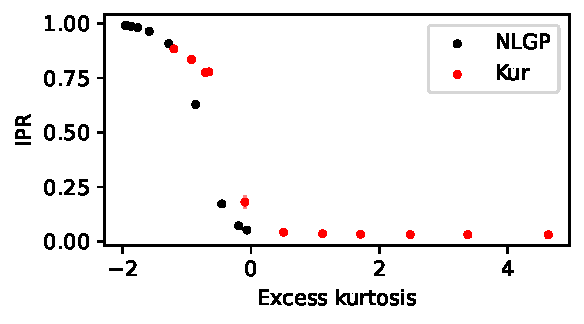
\includegraphics[width=170pt]{rebuttal-figures/replications/kurtosis_vs_ipr_40.pdf}
    \caption{
    IPR \vs excess kurtosis for $\texttt{NLGP}$ and $\texttt{Kur}$ data models, with mean and std.~dev.~across 30 re-initializations for the single-neuron model (\labelcref{item:single-neuron-model});
    error bars are small and may not be visible.
    }
    \label{fig:replications}
    \vspace{-14pt}
\end{wrapfigure}


In \cref{fig:replications}, we validate Claim~\labelcref{thm:localization} first via the single-neuron model (\labelcref{item:single-neuron-model}) with 30 initial conditions trained across a range of excess kurtoses for the $\texttt{NLGP}(g)$ and $\texttt{Kur}(k)$ data models.
We use the inverse participation ratio (IPR), defined in \cref{app:IPR}.
This measure, also used by \textcite{ingrosso2022data}, is large when proportionally few weight dimensions ``participate'' (have large magnitude), and small when weight dimension magnitudes are more uniform.
We see that when $g$ and $k$ assume values that yield a negative excess kurtosis, IPR is close to its maximum of $1.0$, suggesting the weights are localized; if the excess kurtosis is positive, IPR is nearly zero, suggesting the weights are \emph{not} localized.
The IPR is extremely consistent across random initializations, suggesting that localization is determined by data statistics and not initialization.
The trend in IPR \vs excess kurtosis is very similar between the $\texttt{NLGP}(g)$ and $\texttt{Kur}(k)$ data models, demonstrating that excess kurtosis is a primary driver of localization and localization is largely independent from other properties of the data distribution.
\begin{wrapfigure}{l}{0.45\textwidth}
    \centering
    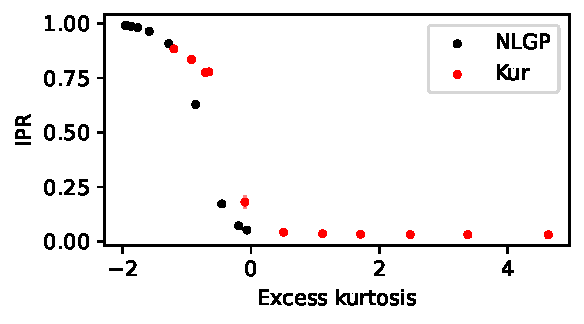
\includegraphics[width=170pt]{rebuttal-figures/replications/kurtosis_vs_ipr_40.pdf}
    \caption{
    IPR \vs excess kurtosis for $\texttt{NLGP}$ and $\texttt{Kur}$ data models, with mean and std.~dev.~across 30 re-initializations for the single-neuron model (\labelcref{item:single-neuron-model});
    error bars are small and may not be visible.
    }
    \label{fig:replications}
    \vspace{-14pt}
\end{wrapfigure}


\Cref{fig:theory} further validates Claim~\labelcref{thm:localization} with specific examples.
We maintain constant initial conditions for our model and train on the \texttt{Ising}, $\texttt{NLGP}(g=0.01)$, and $\texttt{Kur}(k=5)$ data models.
The marginals of the \texttt{Ising} model have an excess kurtosis of $-2$, the smallest possible value for any distribution.
As a result, we see that the amplifier $\varphi$ for \texttt{Ising} (top left) is super-linear (the dark line exceeds the dashed light line for larger $a$), which drives localization via its role in \cref{eq:gradient_flow_early}.
Integrating \cref{eq:gradient_flow_early} with $\varphi$ expanded via a third-order Taylor approximation (red line) yields a similar localized receptive field to that from simulation (two right panels), validating this approximation.

For the remaining distributions (middle and bottom rows) that elicit oscillatory (sinusoidal) weights, 
Claim~\labelcref{thm:localization} is validated due to their positive excess kurtosis.
The dynamical steady state (far right) assumes a more negative value than in the simulation (to the left), 
a difference that is the result of deviations of our \emph{early-time} gradient flow in 
\cref{eq:gradient_flow_early}, but these deviations remain mild enough nevertheless to recover the qualitative structure of the learned receptive field.

\begin{wrapfigure}{l}{0.45\textwidth}
    \centering
    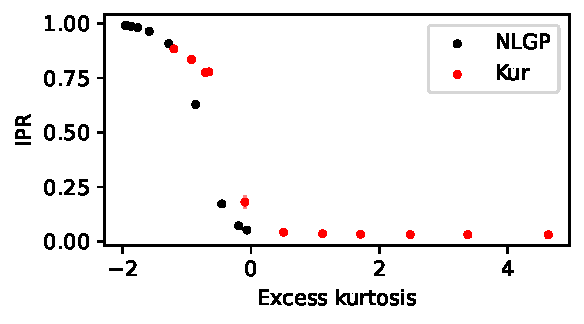
\includegraphics[width=170pt]{rebuttal-figures/replications/kurtosis_vs_ipr_40.pdf}
    \caption{
    IPR \vs excess kurtosis for $\texttt{NLGP}$ and $\texttt{Kur}$ data models, with mean and std.~dev.~across 30 re-initializations for the single-neuron model (\labelcref{item:single-neuron-model});
    error bars are small and may not be visible.
    }
    \label{fig:replications}
    \vspace{-14pt}
\end{wrapfigure}

\subsection{Validating \cref{eq:gradient_flow_early} with localization position prediction}
\label{sec:peak-prediction}
The simulated and integrated receptive fields in \cref{fig:theory} demonstrate that our analytical model is able to meaningfully reproduce localization in receptive fields from neural network training.
For the Ising model, we see that the integration even has a peak in the exact same position as the simulation (at index $i=6$), suggesting precision in our approximation.
Indeed, we simulated the condition in \cref{fig:theory} for the Ising model under 28 different initial conditions (weight initializations), and found that in 26 of them (93\%), the peaks of the integrated and simulated receptive fields matched exactly.
In the two cases where the peaks differed, they did so substantially (see \cref{fig:time} for an example). 

\subsection{Validating Proposition \ref{thm:elliptical}: Elliptical distributions fail to localize}
\label{sec:elliptical-experiments}
Proposition \ref{thm:elliptical} claims that the single-neuron model (\labelcref{item:single-neuron-model})
trained on elliptical data will yield sinusoidal receptive fields, 
subject to a condition on the spectra of $\Sigma_0$ and $\Sigma_1$.
We verify this claim in \cref{fig:elliptical} with three distinct elliptical distributions.
The first, $t_{40}(\nu=3)$, gives preactivations $\langle \mathbf{w}, \mathbf{X} \rangle$ that have \emph{infinite} kurtosis, yet our theory predicts the final receptive field will be sinusoidal.
This is confirmed in \cref{fig:elliptical}, where the learned receptive field is indeed a sinusoid with period 1 and intercept at zero.

We also consider data sampled from the surface of an ellipse, which is done by fixing $R_y \equiv 1$ in \cref{def:elliptical}.
Here, we observe that the learned receptive field is a near-constant function at $-0.04$ (note that $\cos(2\pi \cdot 0 \cdot x) \equiv 1$ is a sinusoid, allowing nonzero intercepts and constant functions).
Finally, we consider an unconventional elliptical distribution where the density of $R$ is given by
$p_R(r) = (4e^{2r+4}) / (e^{2r}+e^{4})^{2} \cdot \mathbbm{1}(r \geq 2)$.
This particular density places most of its mass near $r = 2$ before rapidly falling off, imposing a minimum norm on $\mathbf{X}$ and pushing support near the surface of an ellipse.
This distribution, too, yields an oscillatory steady state, as shown in \cref{fig:elliptical} (right). 
We confirm our visual observations by fitting sinusoids to the final receptive fields and see the relative errors are quite low.

\subsection{Extensions to many-neuron model and ICA}
\label{sec:extensions}

All of our analysis thus far has concerned single-neuron models with ReLU activation and without hidden-to-output or bias terms, assumptions which were made to make our analysis tractable.
Here, we depart from that regime by considering the SCM and the full two-layer network (Model~\labelcref{item:many-neuron-model}).
In \cref{fig:extensions} (left) and (center), we train a SCM with 10 hidden units and sigmoid activation on the $\texttt{Kur}(10)$ and $\texttt{Kur}(4)$ datasets, which have excess kurtoses of $-0.93$ and $3.28$, respectively.
So, based on our single-neuron analysis, we \emph{do} and \emph{do not} expect to see localization for these distributions.
Indeed, this is precisely what we observe in \cref{fig:extensions}, where the receptive fields are sharply localized for the former distribution, while they look like low-frequency oscillations for the latter.

\begin{wrapfigure}{l}{0.45\textwidth}
    \centering
    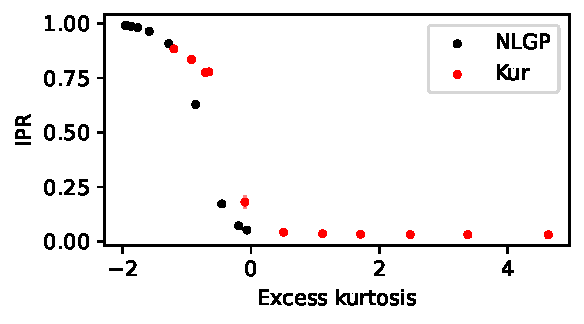
\includegraphics[width=170pt]{rebuttal-figures/replications/kurtosis_vs_ipr_40.pdf}
    \caption{
    IPR \vs excess kurtosis for $\texttt{NLGP}$ and $\texttt{Kur}$ data models, with mean and std.~dev.~across 30 re-initializations for the single-neuron model (\labelcref{item:single-neuron-model});
    error bars are small and may not be visible.
    }
    \label{fig:replications}
    \vspace{-14pt}
\end{wrapfigure}

In \cref{fig:multi-neuron}, we train many-neuron models with $N=40$ input units and $K=10$ hidden units, where all weights are learnable.
In general, adding flexibility in the second layer leads to more varied structure in the first layer.
We train on $\texttt{Kur}(4)$ (top), which has an excess kurtosis of $3.28$, and $\texttt{Kur}(30)$ (bottom), which has an excess kurtosis of $-1.17$.
The receptive fields from the former are not localized, as in the single-neuron model; however, they appear more like high-frequency oscillations than low-frequency sinusoids.
For $\texttt{Kur}(30)$, where we expect localization, we see that the first three receptive fields exhibit localization, but less so than for a single neuron.
Importantly, not all receptive fields are localized,
a result of a variable second-layer weight effectively changing the variance $\sigma^2$ in the third-derivative term in Lemma~\labelcref{lem:varphi}.

We further compare these predictions against ICA, another framework that has been used to model receptive fields in visual cortex.
We train on the $\texttt{Kur}(3)$ dataset, which has marginals with excess kurtosis $7.66$, fitting 10 components using the FastICA implementation from scikit-learn \parencite{hyvarinen2000independent,scikit-learn}.
We observe in \cref{fig:extensions} (right) that we learn localized receptive fields; this contrasts our neural network models, which require negative excess kurtosis.
This stems from ICA's objective to maximize non-Gaussianity, regardless of how specifically it is done.
The sign of the excess kurtosis is irrelevant, so long as it is nonzero.
This deviation between our analytical model and ICA is an interesting avenue for future study, perhaps by validation with natural images.
